% !TEX encoding = UTF-8
\chapter{Triển khai và kiểm chứng kiến trúc Zero Trust}

%==============================================================================
% 3.1 MÔ TẢ HỆ THỐNG VÀ PHẠM VI THỰC NGHIỆM
%==============================================================================
\section{Mô tả hệ thống và phạm vi thực nghiệm}

Hệ thống thực nghiệm mang tên \texttt{job7189} là một nền tảng tuyển dụng trực tuyến được thiết kế theo kiến trúc Microservices. Hệ thống bao gồm 7 vi dịch vụ nghiệp vụ độc lập: \texttt{identity}, \texttt{workspace}, \texttt{job}, \texttt{hiring}, \texttt{candidate}, \texttt{communication}, và \texttt{storage}. Các dịch vụ này giao tiếp nội bộ thông qua HTTP/REST và hệ thống hàng đợi thông điệp, đồng thời sử dụng các cơ sở dữ liệu phân tán (MySQL, Redis, Kafka).


Các luồng tích hợp nghiệp vụ và sơ đồ phân vùng dữ liệu của hệ thống được mô tả khái quát qua các hình vẽ ngữ cảnh hệ thống (Hình~\ref{fig:intro_context_job7189}), kiến trúc ứng dụng (Hình~\ref{fig:intro_container_job7189}) và sơ đồ kết nối dữ liệu (Hình~\ref{fig:intro_containerdb_job7189}).

\begin{figure}[H]
  \centering
  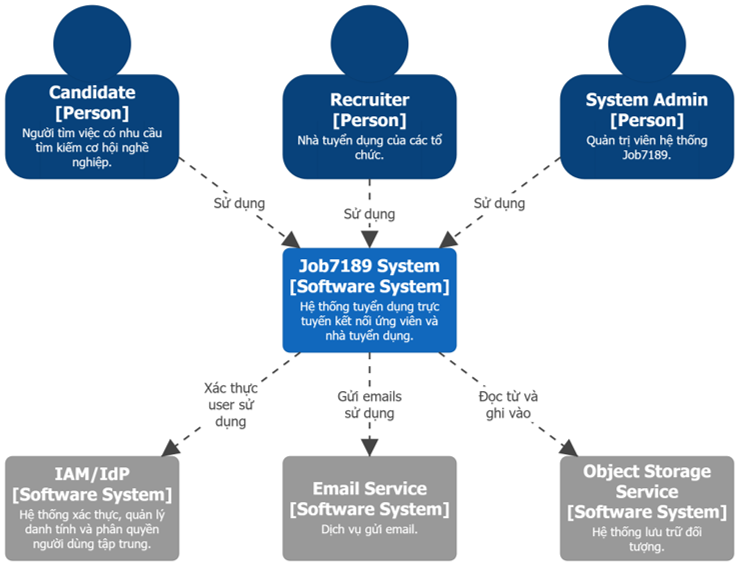
\includegraphics[width=0.88\textwidth]{images/context.png}
  \caption{Sơ đồ ngữ cảnh hệ thống Job7189}
  \label{fig:intro_context_job7189}
\end{figure}

\begin{figure}[H]
  \centering
  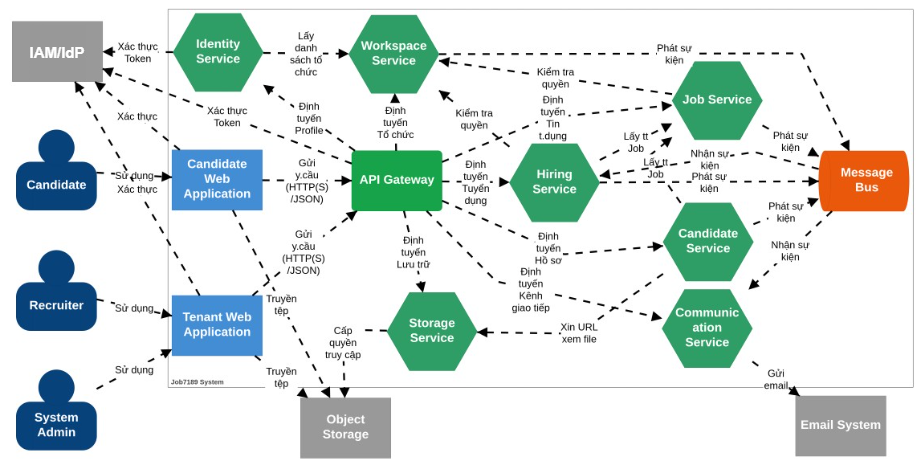
\includegraphics[width=0.92\textwidth]{images/container.png}
  \caption{Kiến trúc container của hệ thống Job7189 (góc nhìn nghiệp vụ)}
  \label{fig:intro_container_job7189}
\end{figure}

\begin{figure}[H]
  \centering
  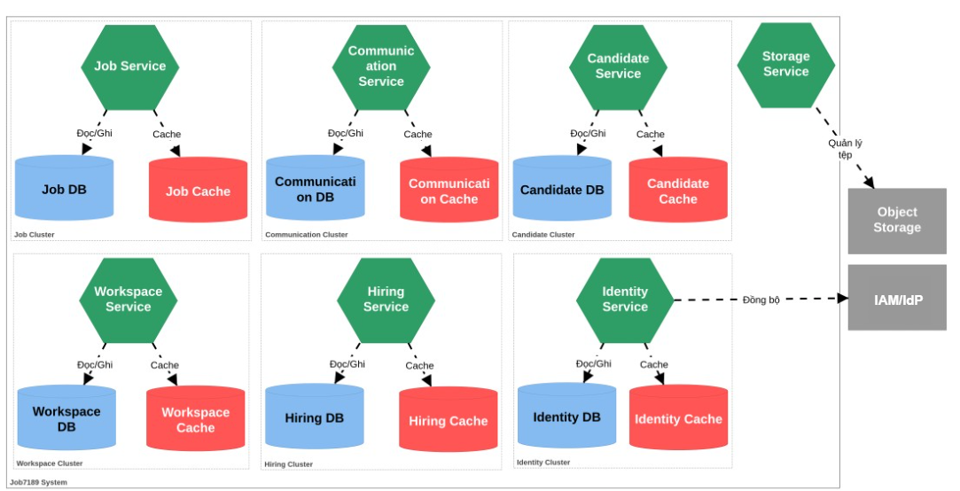
\includegraphics[width=0.92\textwidth]{images/containerdb.png}
  \caption{Kiến trúc container của hệ thống Job7189 (góc nhìn dữ liệu)}
  \label{fig:intro_containerdb_job7189}
\end{figure}

\textbf{Phạm vi thực nghiệm:} Đồ án tập trung hiện thực hóa kiến trúc Zero Trust ở phía máy chủ (Server-side) và khối lượng công việc (Workload). Các mục tiêu chính bao gồm: định danh thực thể, phân đoạn mạng vi mô, quản lý thông tin xác thực động và giám sát thời điểm chạy. 

\textbf{Loại trừ có chủ đích:} Việc kiểm tra tư thế bảo mật của thiết bị người dùng cuối (Client Device Posture) và các cơ chế đánh giá truy cập liên tục nâng cao tích hợp GitOps (CAEP/GitOps) nằm ngoài phạm vi của nguyên mẫu (PoC) này.

%==============================================================================
% 3.2 KHẢO SÁT HIỆN TRẠNG (DISCOVERY)
%==============================================================================
\section{Khảo sát hiện trạng hệ thống (Discovery)}

Tuân thủ nguyên tắc triển khai của tiêu chuẩn NIST SP 800-207 (Bước 1 đến Bước 3), trước khi áp dụng chính sách cưỡng chế, hệ thống cần trải qua giai đoạn khảo sát toàn diện. Kết quả khảo sát là đầu vào bắt buộc để xây dựng tập luật kiểm soát truy cập sát với thực tế.

\begin{itemize}[itemsep=6pt, parsep=0pt]
    \item \textbf{Kiểm kê chủ thể (Subjects):} Bao gồm người dùng cuối được quản lý qua Keycloak Realm \texttt{job7189}; quản trị viên hệ thống qua Realm \texttt{7189\_internal}; và các thực thể phi con người (7 vi dịch vụ, các tác vụ CronJob, bộ điều khiển PDP).
    
    \item \textbf{Kiểm kê tài sản (Assets):} Cụm thực nghiệm gồm 4 máy chủ (1 Control Plane, 3 Worker Nodes) kết nối qua mạng riêng ảo Tailscale. Tài sản phần mềm bao gồm 7 vi dịch vụ nghiệp vụ, 7 bản sao Redis, cụm MySQL và Kafka.
    
    \item \textbf{Bản đồ luồng dữ liệu (Data Flows):} Thay vì phỏng đoán luồng giao tiếp dựa trên mã nguồn, đồ án sử dụng công cụ Hubble chạy ở \textbf{chế độ ghi nhận (Audit mode)}. Cơ chế này cho phép bắt toàn bộ lưu lượng mạng thực tế sinh ra trong quá trình hệ thống hoạt động bình thường mà không làm rớt gói tin. Từ dữ liệu đo lường từ xa (telemetry) thu thập được, hệ thống vẽ ra bản đồ luồng dữ liệu chính xác gồm 3 trục: (1) Luồng Bắc-Nam từ API Gateway; (2) Luồng Đông-Tây giữa các vi dịch vụ; (3) Luồng truy xuất cơ sở dữ liệu. Đây là căn cứ kỹ thuật trực tiếp để định nghĩa các chính sách phân đoạn mạng vi mô ở giai đoạn sau.
\end{itemize}

%==============================================================================
% 3.3 THIẾT KẾ ZERO TRUST CHO JOB7189
%==============================================================================
\section{Thiết kế Zero Trust cho hệ thống job7189}

\subsection{Phân bổ không gian tên (Namespace)}

Nhằm thiết lập ranh giới cách ly logic ban đầu, khối lượng công việc được phân bổ vào 7 không gian tên độc lập dựa trên mức độ rủi ro và chức năng vận hành.

% [CHÈN C3 CŨ VÀO ĐÂY: Sơ đồ TikZ hoặc hình ảnh mô tả phân bổ Namespace (fig:c3_namespace_map)]

\subsection{Lộ trình triển khai 5 giai đoạn}

Quá trình cài đặt tuân theo lộ trình chuyển đổi đề xuất tại Mục 2.3.3 (bảy bước NIST SP 800-207, nguyên tắc 'audit trước $\rightarrow$ enforce sau'), được cụ thể hóa thành năm giai đoạn thực thi trên hệ thống \texttt{job7189}:

\begin{enumerate}[itemsep=6pt, parsep=0pt]
    \item \textbf{Giai đoạn 0 (Baseline hạ tầng):} Triển khai hạ tầng và ứng dụng cơ bản chưa có cơ chế Zero Trust.
    \item \textbf{Giai đoạn 1 (Quản lý tài nguyên \& định danh):} Cài đặt SPIRE, cert-manager và Keycloak để thiết lập gốc tin cậy.
    \item \textbf{Giai đoạn 2 (Chế độ Audit):} Triển khai các điểm thực thi (Cilium, Gatekeeper, Tetragon) ở chế độ ghi nhận, thu thập dữ liệu luồng.
    \item \textbf{Giai đoạn 3 (Mở rộng Cưỡng chế - Enforce):} Kích hoạt chính sách chặn mặc định, áp dụng luật mạng tường minh.
    \item \textbf{Giai đoạn 4 (Thích ứng):} Kích hoạt vòng lặp phản hồi của bộ điều khiển PDP và cấp phát bí mật động qua Vault.
\end{enumerate}

%==============================================================================
% 3.4 TRIỂN KHAI 5 THÀNH PHẦN CHỨC NĂNG
%==============================================================================
\section{Triển khai 5 thành phần chức năng}

Triển khai bám sát năm thành phần chức năng (TC1–TC5) đã đề xuất ở Chương 2. Trong đó, hệ thống quản lý bí mật (Vault) được trình bày với tư cách là Bộ điều phối chính sách thuộc TC3, không phải một thành phần tách rời.

% [CHÈN C3 CŨ VÀO ĐÂY: Sơ đồ fig:c3_5layer_design (Vẽ lại 5 hộp theo thứ tự luồng TC1->TC5, Vault chui vào TC3, Cosign vào TC2, PDP loop vào TC5)]

\subsection{TC1 — Định danh và Xác thực}
\begin{itemize}[itemsep=6pt, parsep=0pt]
    \item \textbf{Công nghệ:} Keycloak (Người dùng) và SPIRE (Workload).
    \item \textbf{Cấu hình:} SPIRE Server lưu trữ gốc tin cậy. SPIRE Agent trên mỗi Node thực hiện chứng thực khối lượng công việc, cấp phát chứng chỉ X.509 SVID với thời gian sống ngắn.
    \item \textbf{Chế độ lỗi:} Nếu SPIRE Server gián đoạn, các SVID hiện tại vẫn hợp lệ cho đến khi hết hạn. Workload mới không thể khởi động khi chưa có SVID hợp lệ — đây là hành vi từ chối an toàn có chủ đích.
\end{itemize}

\subsection{TC2 — Đánh giá tư thế và tình báo đe dọa}
\begin{itemize}[itemsep=6pt, parsep=0pt]
    \item \textbf{Công nghệ:} Trivy Operator, Sigstore (Cosign), và FireHOL.
    \item \textbf{Cấu hình:} Trivy liên tục quét lỗ hổng sinh ra \texttt{VulnerabilityReport}. Tại cổng nạp (Admission), Sigstore policy-controller kiểm tra tính hợp lệ của chữ ký image. Trong phạm vi PoC, cơ chế này đang hoạt động ở chế độ cảnh báo (\texttt{mode=warn}). Danh sách IP độc hại từ FireHOL được đồng bộ vào \texttt{CiliumCIDRGroup}.
\end{itemize}

\subsection{TC3 — Ra quyết định (PE + PA + Vault)}
\begin{itemize}[itemsep=6pt, parsep=0pt]
    \item \textbf{Công nghệ:} Bộ điều khiển PDP (Python/Kopf) và HashiCorp Vault.
    \item \textbf{Cấu hình:} PDP Controller đóng vai trò Động cơ chính sách (PE), liên tục đọc dữ liệu từ TC2 và TC5 để tính toán mức độ rủi ro, gán nhãn \texttt{score-bucket} cho Pod. Vault đóng vai trò Bộ điều phối (PA), tiếp nhận định danh JWT-SVID của Pod để ra quyết định cấp phát thông tin xác thực cơ sở dữ liệu động (JIT).
\end{itemize}

\subsection{TC4 — Thực thi chính sách đa tầng}
\begin{itemize}[itemsep=6pt, parsep=0pt]
    \item \textbf{Công nghệ:} Kong Gateway, Cilium eBPF, OPA Gatekeeper, Tetragon.
    \item \textbf{Cấu hình:} Kong kiểm tra JWT tại biên. Cilium thực thi chính sách mạng nội bộ dựa trên nhãn định danh. OPA Gatekeeper chặn các cấu hình sai lệch. Tetragon can thiệp trực tiếp tại Kernel. Động tác tiêm mật khẩu động vào Pod được thực hiện bởi Vault Agent sidecar (mount vào \texttt{tmpfs}).
\end{itemize}

\subsection{TC5 — Quan sát và Phản hồi}
\begin{itemize}[itemsep=6pt, parsep=0pt]
    \item \textbf{Công nghệ:} EFK Stack, Prometheus, Hubble.
    \item \textbf{Cấu hình:} Hubble ánh xạ gói tin mạng với định danh thực thể. Toàn bộ sự kiện an ninh được đẩy về Elasticsearch. Dữ liệu này đóng vòng phản hồi về TC3 để hệ thống tự động điều chỉnh chính sách cưỡng chế.
\end{itemize}

%==============================================================================
% 3.5 KIỂM CHỨNG THỰC NGHIỆM
%==============================================================================
\section{Kiểm chứng thực nghiệm các kịch bản tấn công}

% [CHÈN C3 CŨ VÀO ĐÂY: Dán toàn bộ Kịch bản 1 đến Kịch bản 6 của bạn vào đây. Giữ đúng thứ tự KB1 = Tetragon, KB2 = Vault... kèm theo các block code/log thực tế. Nhớ bổ sung log Exit Code 137 cho Tetragon như đã thống nhất.]

%==============================================================================
% 3.6 ĐÁNH GIÁ TỔNG HỢP VÀ HẠN CHẾ
%==============================================================================
\section{Đánh giá tổng hợp và hạn chế}

Đồ án kiểm chứng 6 kịch bản tấn công-phòng thủ toàn trình (KB1–KB6) với nhật ký thực tế, bao phủ 10 kỹ thuật MITRE ATT\&CK for Containers. Bảng \ref{tab:c3_mitre_summary} liệt kê tổng hợp 17 kỹ thuật tấn công, bao gồm 10 kỹ thuật đã kiểm chứng thực tế và 7 kỹ thuật ở mức độ định hướng thiết kế, nhằm đánh giá độ phủ phòng thủ toàn diện của kiến trúc chứ không chỉ giới hạn ở phần đã chạy.

% [CHÈN C3 CŨ VÀO ĐÂY: Dán Bảng 17 dòng MITRE vào đây. Nhớ có cột 'Mức minh chứng' (Đã kiểm chứng [A] / Một phần / Thiết kế)]

\subsection{Mức độ cưỡng chế thực tế của hệ thống}

Để đảm bảo tính trung thực khoa học, Bảng \ref{tab:enforcement_level} đối chiếu trạng thái cấu hình thực tế của cụm thực nghiệm (tính đến thời điểm báo cáo) so với lý thuyết thiết kế. Trong phạm vi PoC, một số cơ chế (như Gatekeeper, Cosign) hoạt động ở chế độ ghi nhận (monitor mode) theo đúng bước 6 của lộ trình NIST SP 800-207 nhằm tránh gián đoạn dịch vụ hợp lệ.

\begin{table}[H]
\centering
\caption{Mức độ cưỡng chế thực tế của các cơ chế bảo mật}
\label{tab:enforcement_level}
\renewcommand{\arraystretch}{1.3}
\begin{tabularx}{\textwidth}{|p{3.5cm}|X|X|}
\hline
\textbf{Cơ chế / Công cụ} & \textbf{Trạng thái thực tế trên cụm} & \textbf{Ghi nhận trong báo cáo} \\
\hline
mTLS (Cilium) & \texttt{mesh-auth-enabled=true} (Dùng SVID) & Đã bật. \\
\hline
Mã hóa L3 (WireGuard) & \texttt{enable-wireguard=false} & Bắt buộc tắt để tránh xung đột mã hóa kép do Tailscale đã đảm nhận L3. \\
\hline
Giám sát Runtime (Tetragon) & v1.7.0, \texttt{Sigkill enforce} ở 4 namespace (có TracingPolicy). & Ngắt tại nhân, với TracingPolicy tương ứng. \\
\hline
Chữ ký số (Cosign) & 3 ClusterImagePolicy đang ở \texttt{mode=warn}. & WARN — chuyển enforce ở giai đoạn sau. Chốt cứng dựa vào digest-pin. \\
\hline
Kiểm soát cổng nạp (Gatekeeper) & Hoạt động ở chế độ \texttt{dryrun} (Audit), chỉ \texttt{zta-block-host-mounts = deny}. & Phần lớn audit; chốt cứng là digest-pin + netpol + seccomp. \\
\hline
Trivy Operator & Đang chạy, $\sim$5 VulnerabilityReport. & Posture feed hoạt động. \\
\hline
Threat-Intel & CIDRGroup $\sim$2000 CIDR, CronJob active. & Đã đồng bộ. \\
\hline
Vòng lặp PDP & Thành phần đủ, chưa demo e2e (mọi pod đang ở mức high). & Đã hiện thực một phần — cần pod điểm thấp để minh chứng. \\
\hline
\end{tabularx}
\end{table}

\subsection{Hạn chế của nguyên mẫu thực nghiệm}

Mô hình điểm tin cậy và vòng lặp phản hồi PDP hiện tại đã được triển khai thành phần điều khiển (controller), tuy nhiên chưa được kiểm chứng tự động toàn trình (end-to-end) do mọi khối lượng công việc hiện tại đều đạt điểm tin cậy cao. Việc minh chứng kịch bản cô lập tự động đòi hỏi phải chủ động tiêm một vùng chứa mang lỗ hổng nghiêm trọng vào hệ thống.

Bên cạnh đó, trục đánh giá \textit{Phân cấp dịch vụ (Service Tier)} đã được đọc từ nhãn của Kubernetes nhưng chưa được tích hợp vào hàm tính điểm. Trục \textit{Khả năng khai thác (Exploitability)} hiện đang dừng ở mức định hướng thiết kế, do báo cáo của Trivy Operator chưa hỗ trợ trực tiếp thông tin về mã khai thác công khai, đòi hỏi hệ thống phải tích hợp thêm nguồn cấp dữ liệu từ CISA KEV hoặc EPSS trong tương lai.